\subsection{22 августа. Д.р. Джалпаккол}
\textit{Метеоусловия: утром, днём ясно, вечером~--- переменная облачность, тепло. Ночью сильная гроза.}

\begin{figure}[h!]
	\centering
	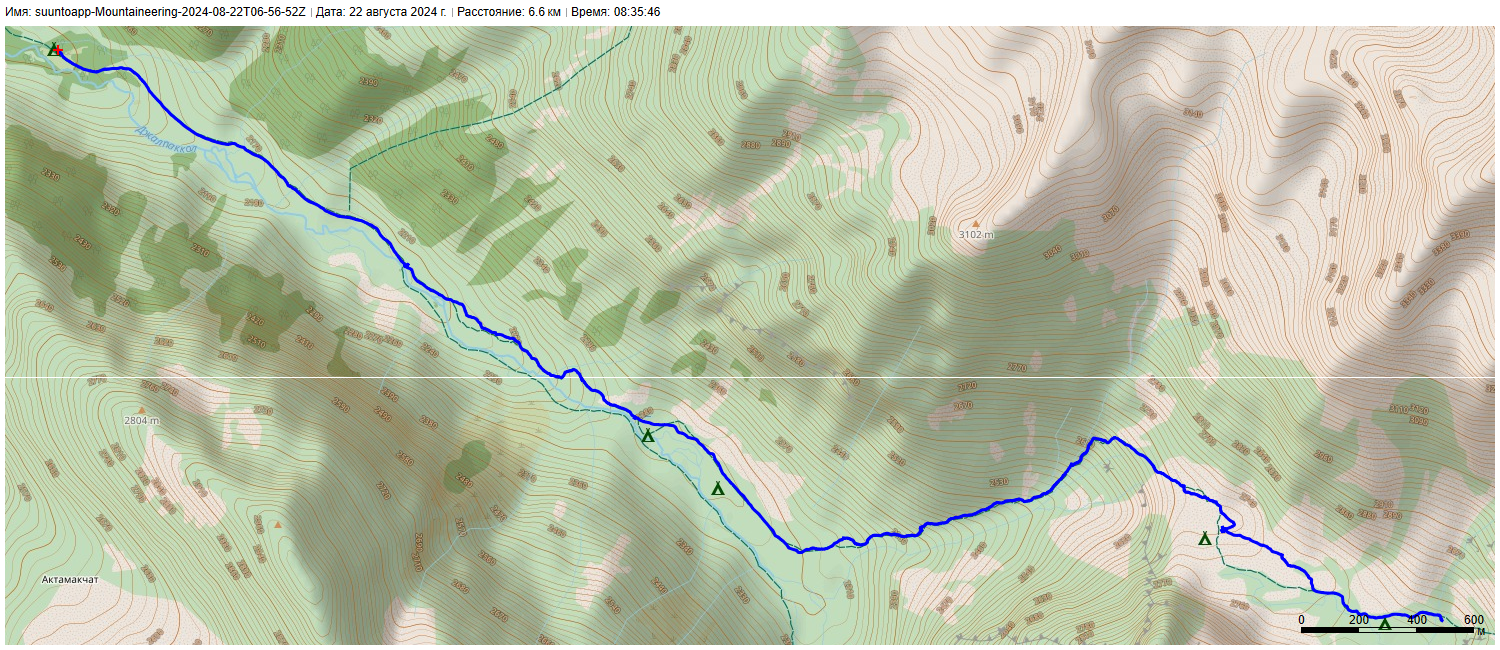
\includegraphics[angle=0, width=0.7\linewidth]{../pics/mini_maps/22}
	\label{fig:mini_22}
\end{figure}


\begin{figure}[h!]
	\centering
	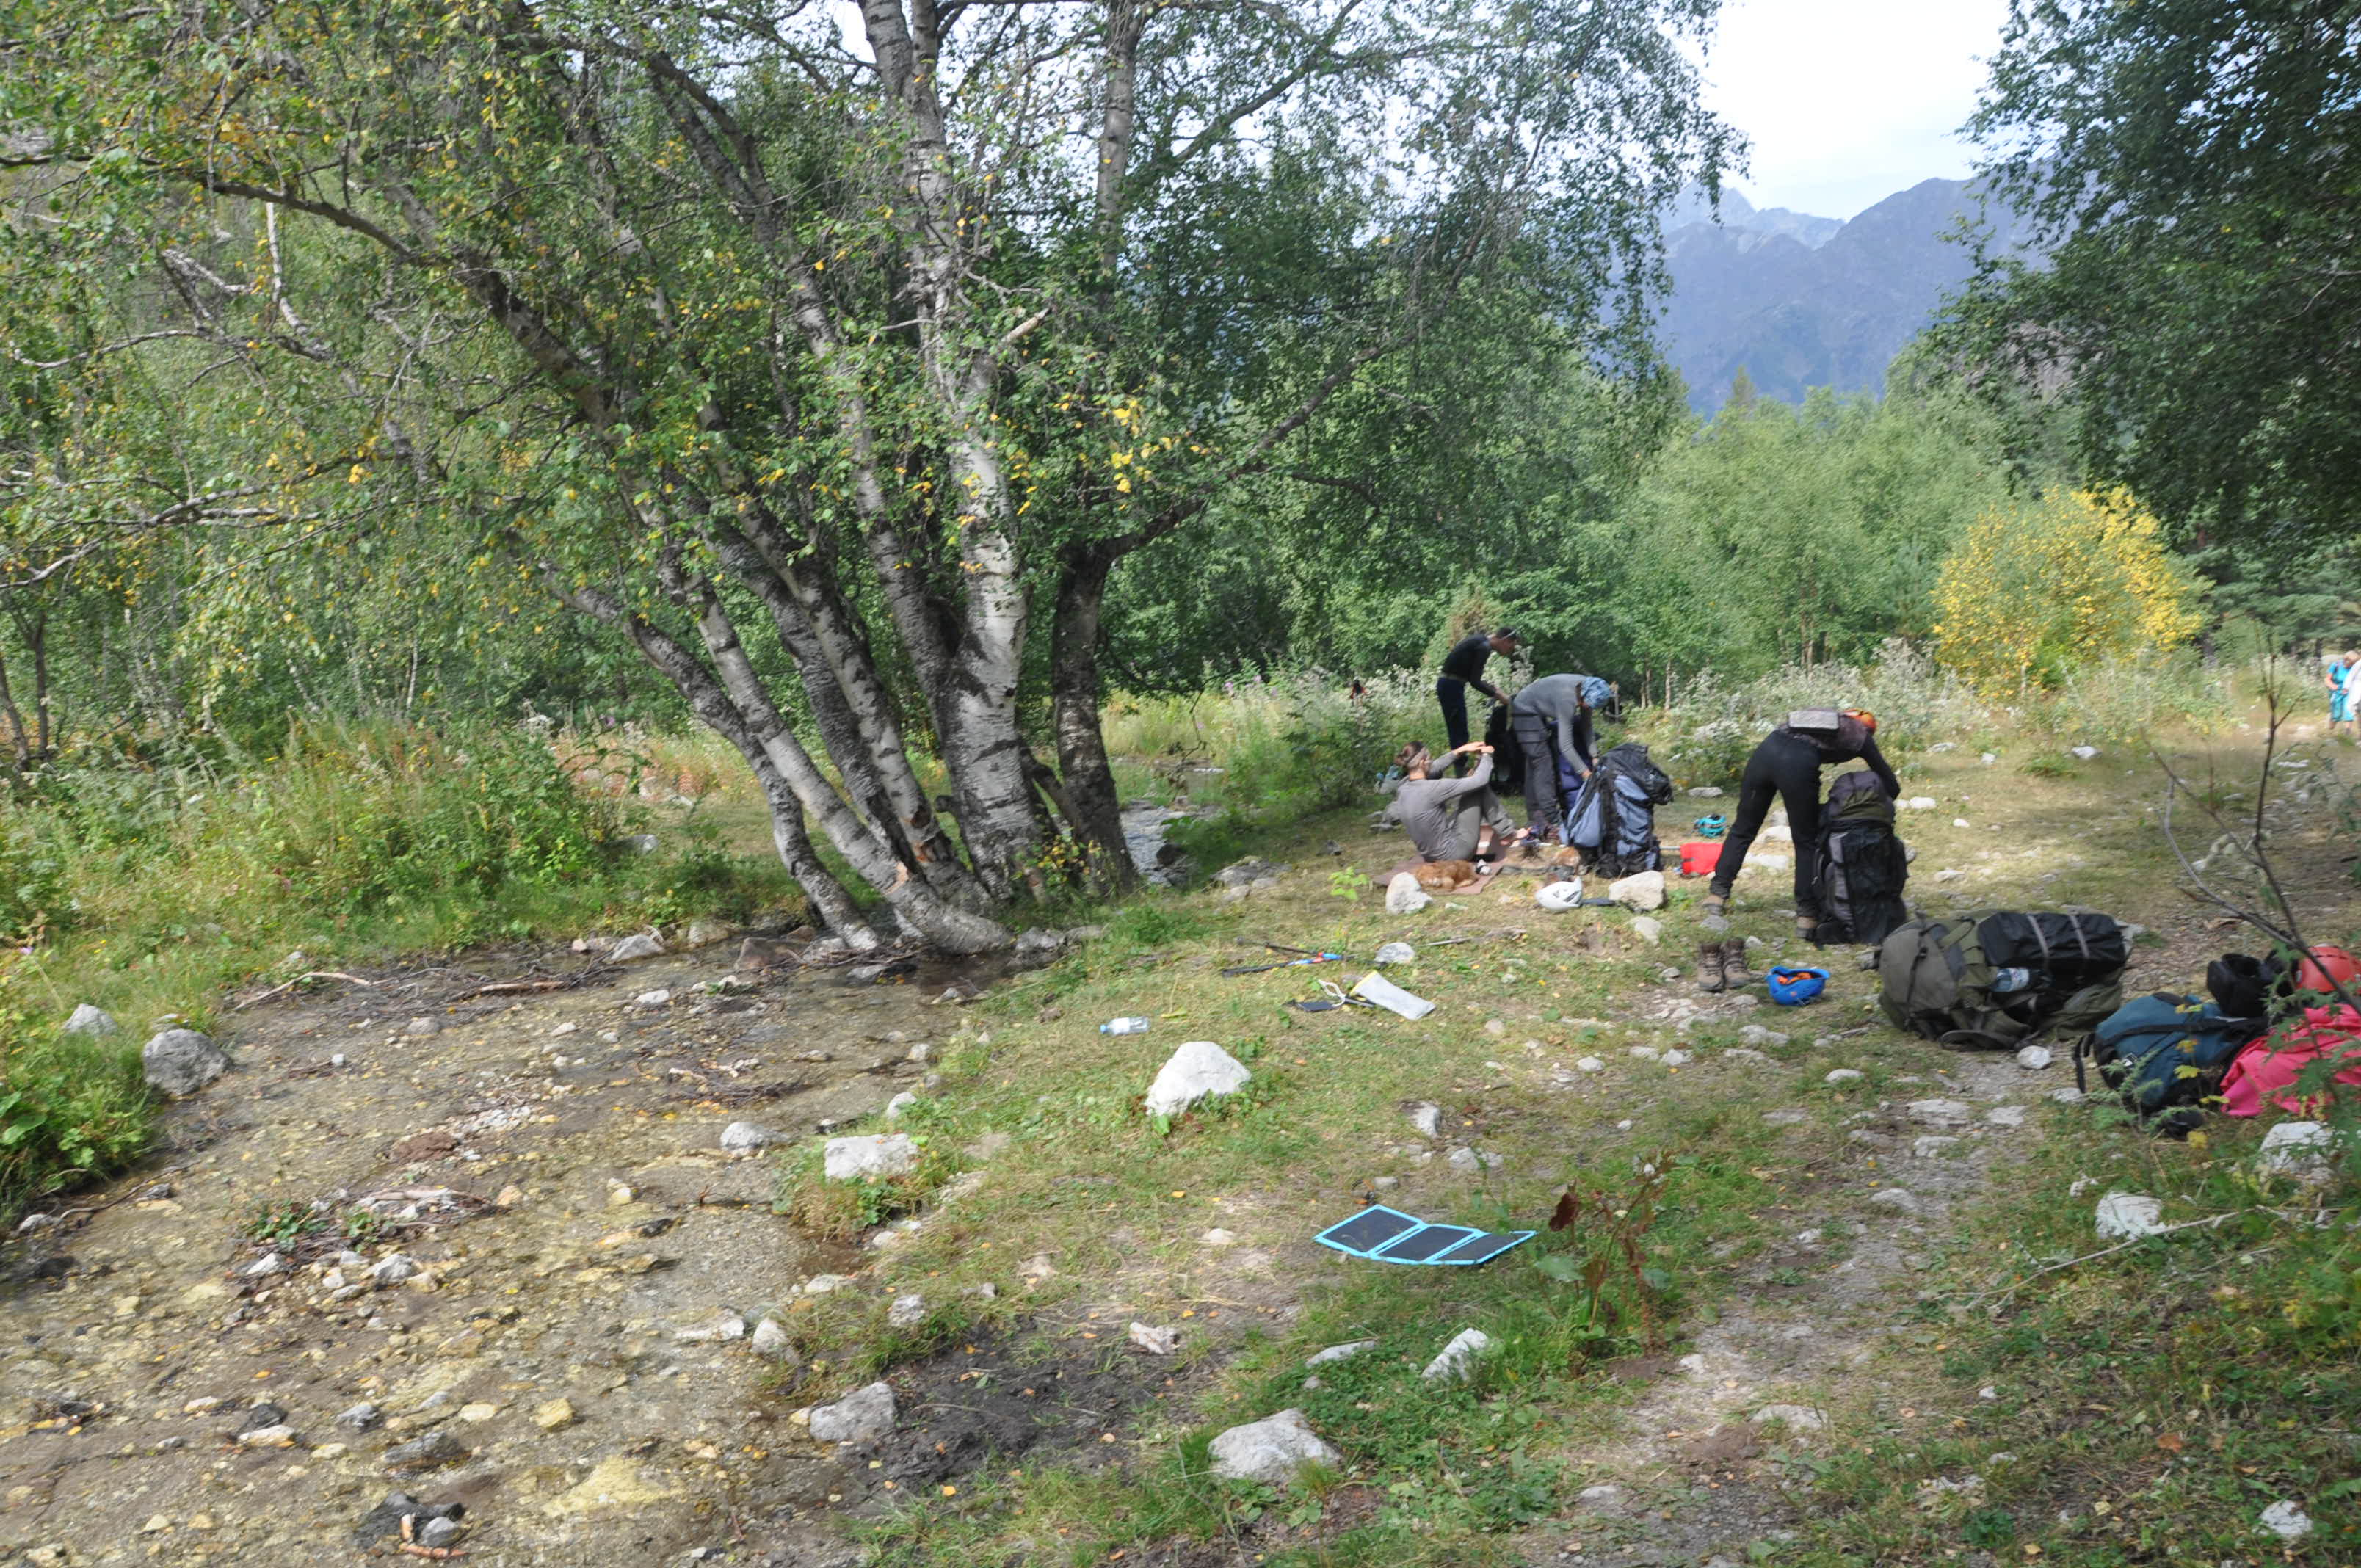
\includegraphics[width=0.7\linewidth]{../pics/DSC_1181}
	\caption{Место ночёвки 21-22.08. Утренние сборы}
	\label{fig:DSC_1181}
\end{figure}


Из-за позднего завершения ходового дня накануне устроили подъём достаточно поздно, в 08:00, и выходим в 10:00 (рис. \ref{fig:DSC_1181}). Шли по правому берегу р. Джалпаккол, не переходя на левый берег у коша N 43.296700\degree,~E 42.046662\degree. Тропа здесь хорошо набита, место часто посещаемо: обогнали группу пенсионеров, поднимавшихся от т/б <<Глобус>> к водопадам д.р. Кичкинекол Джалпаккольский. По пути встречались бесконечные поляны крокусов (рис. \ref{fig:IMG_20240822_101505}).

\begin{figure}[h!]
	\centering
	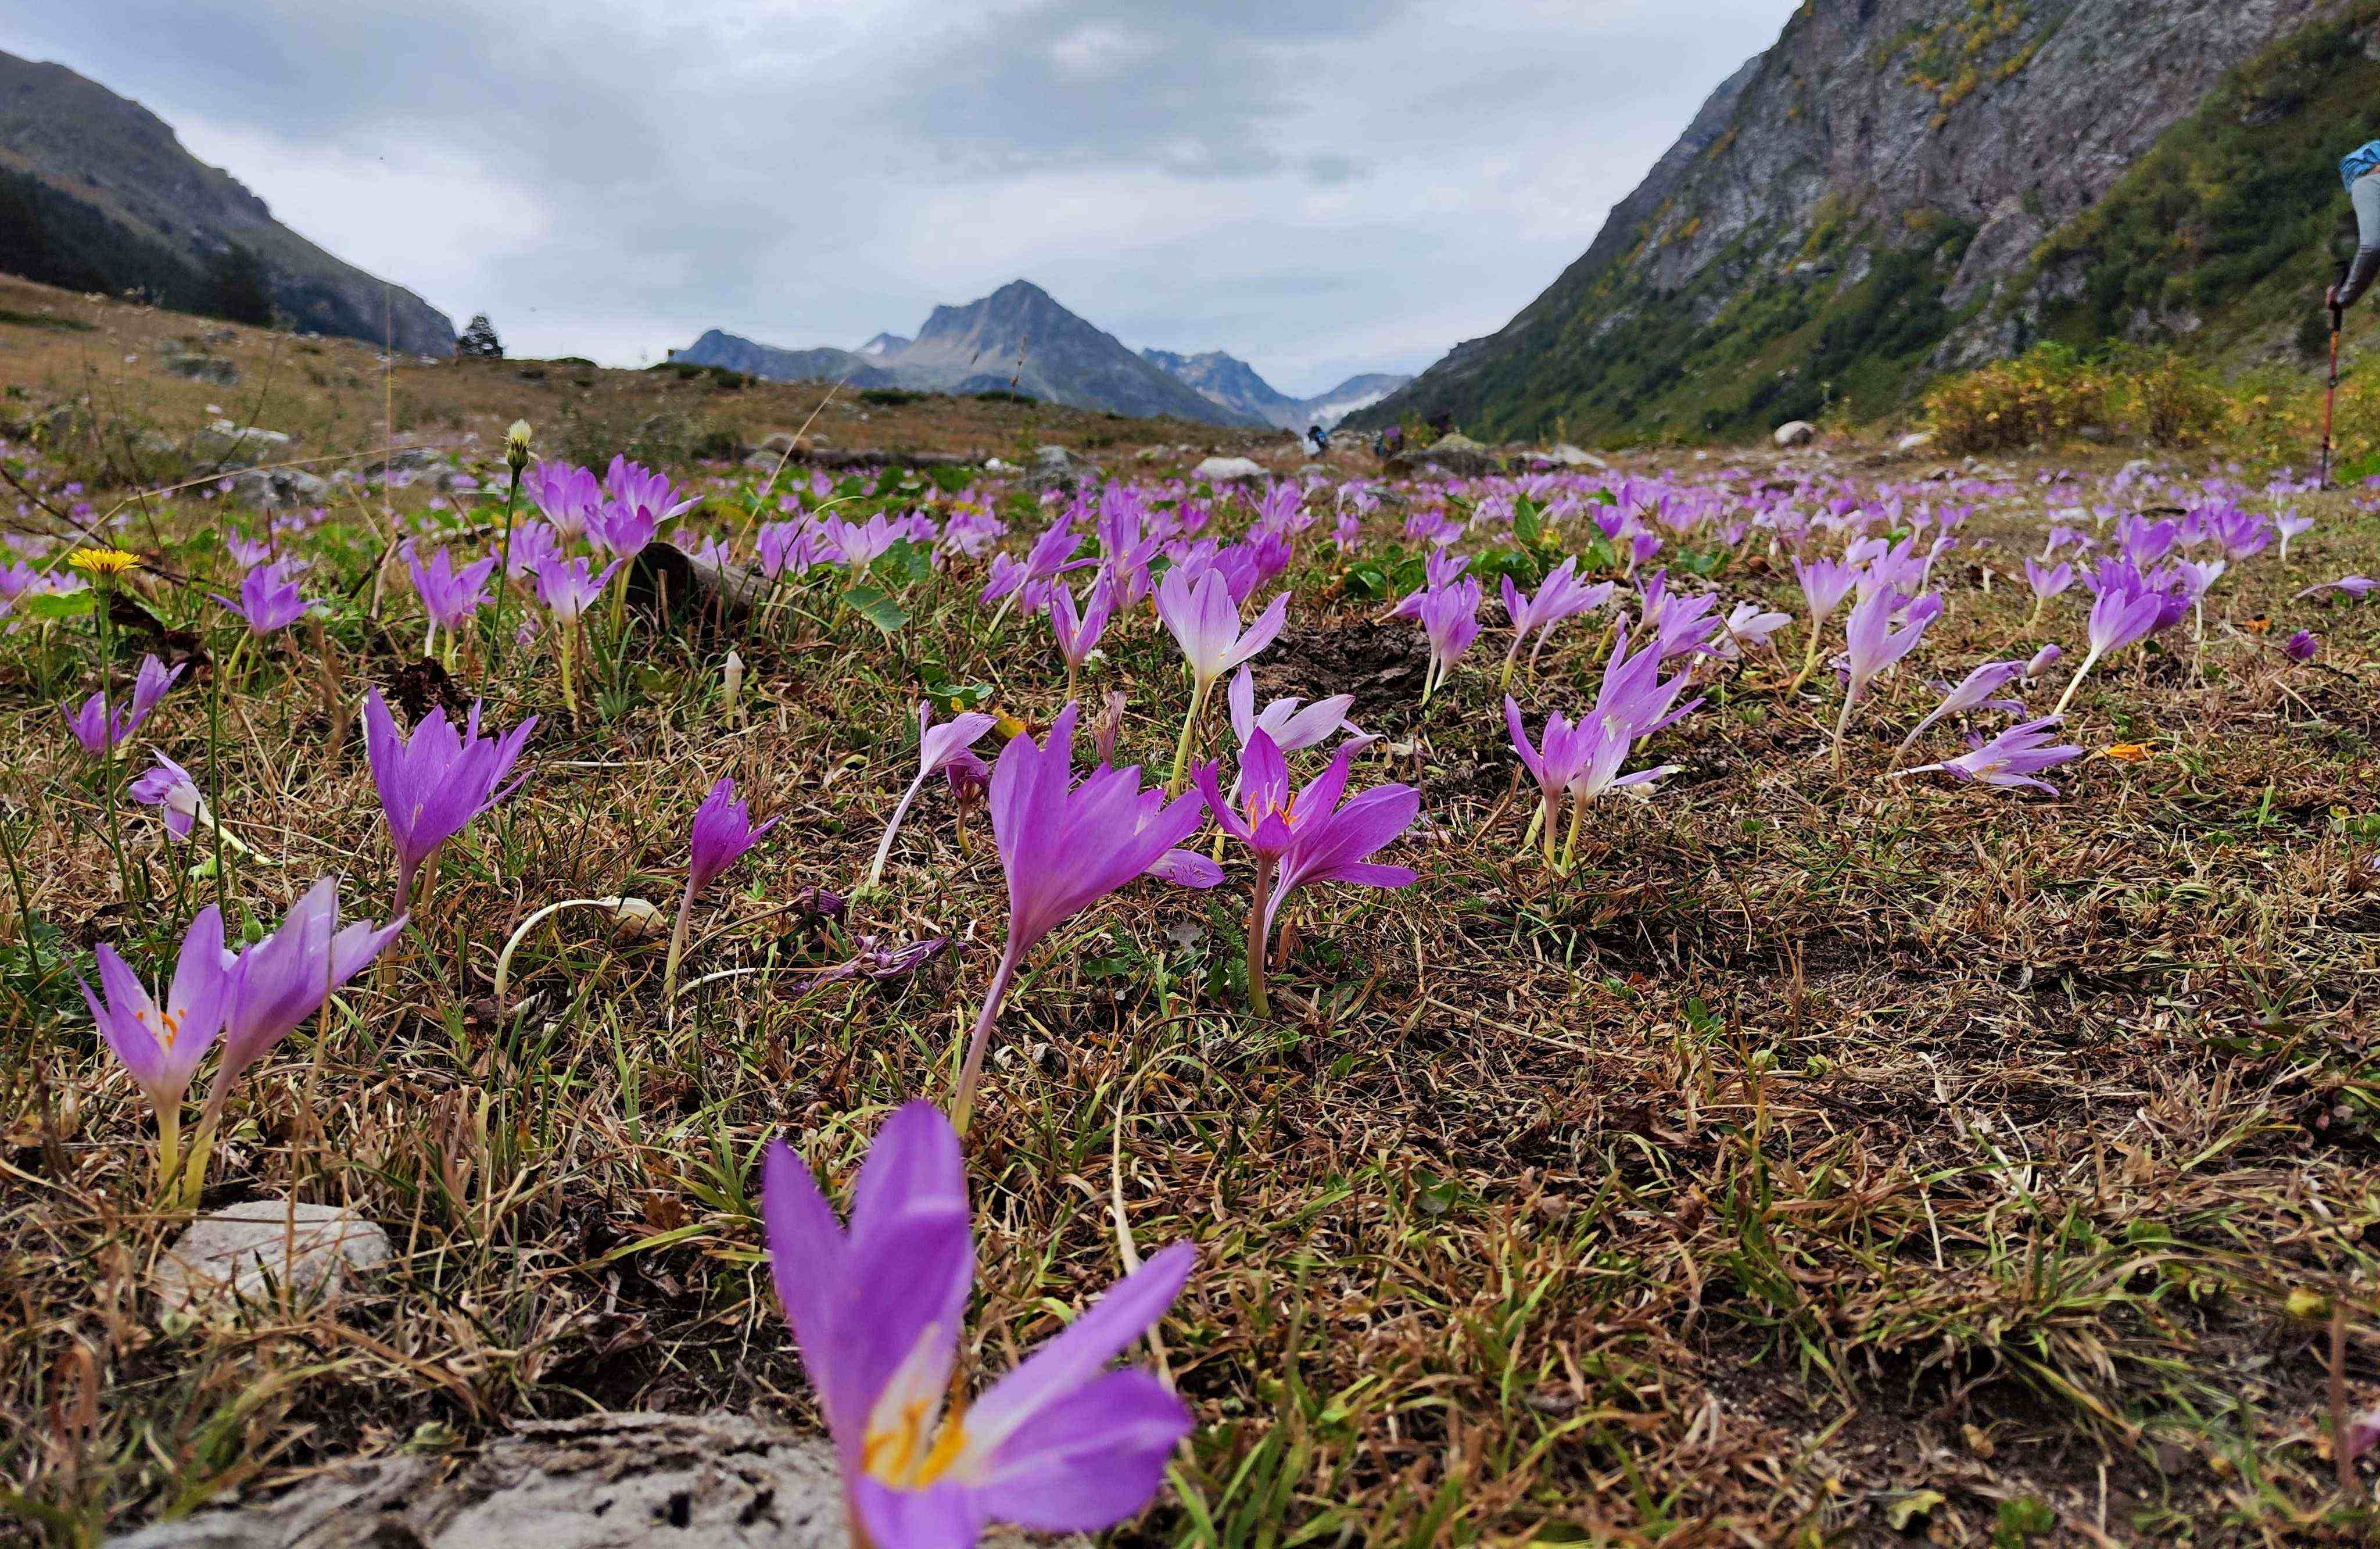
\includegraphics[width=0.7\linewidth]{../pics/IMG_20240822_101505}
	\caption{Крокусы в д.р. Джалпаккол}
	\label{fig:IMG_20240822_101505}
\end{figure}

В 11:45 дошли до развилки: направо пхд~--- верховья д.р. Джалпаккол, налево~--- д.р. Кичкинекол Джалпаккольский. Панорама здесь весьма живописная: плоская долина Джалппаккола (откуда и карачаевское название) как на ладони, в ущелье Кичкинекола шумит река, впереди открывается вид на хребет Куршо. Остановились на фотопривал (рис. \ref{fig:DJI_0830}).

\begin{figure}[h!]
	\centering
	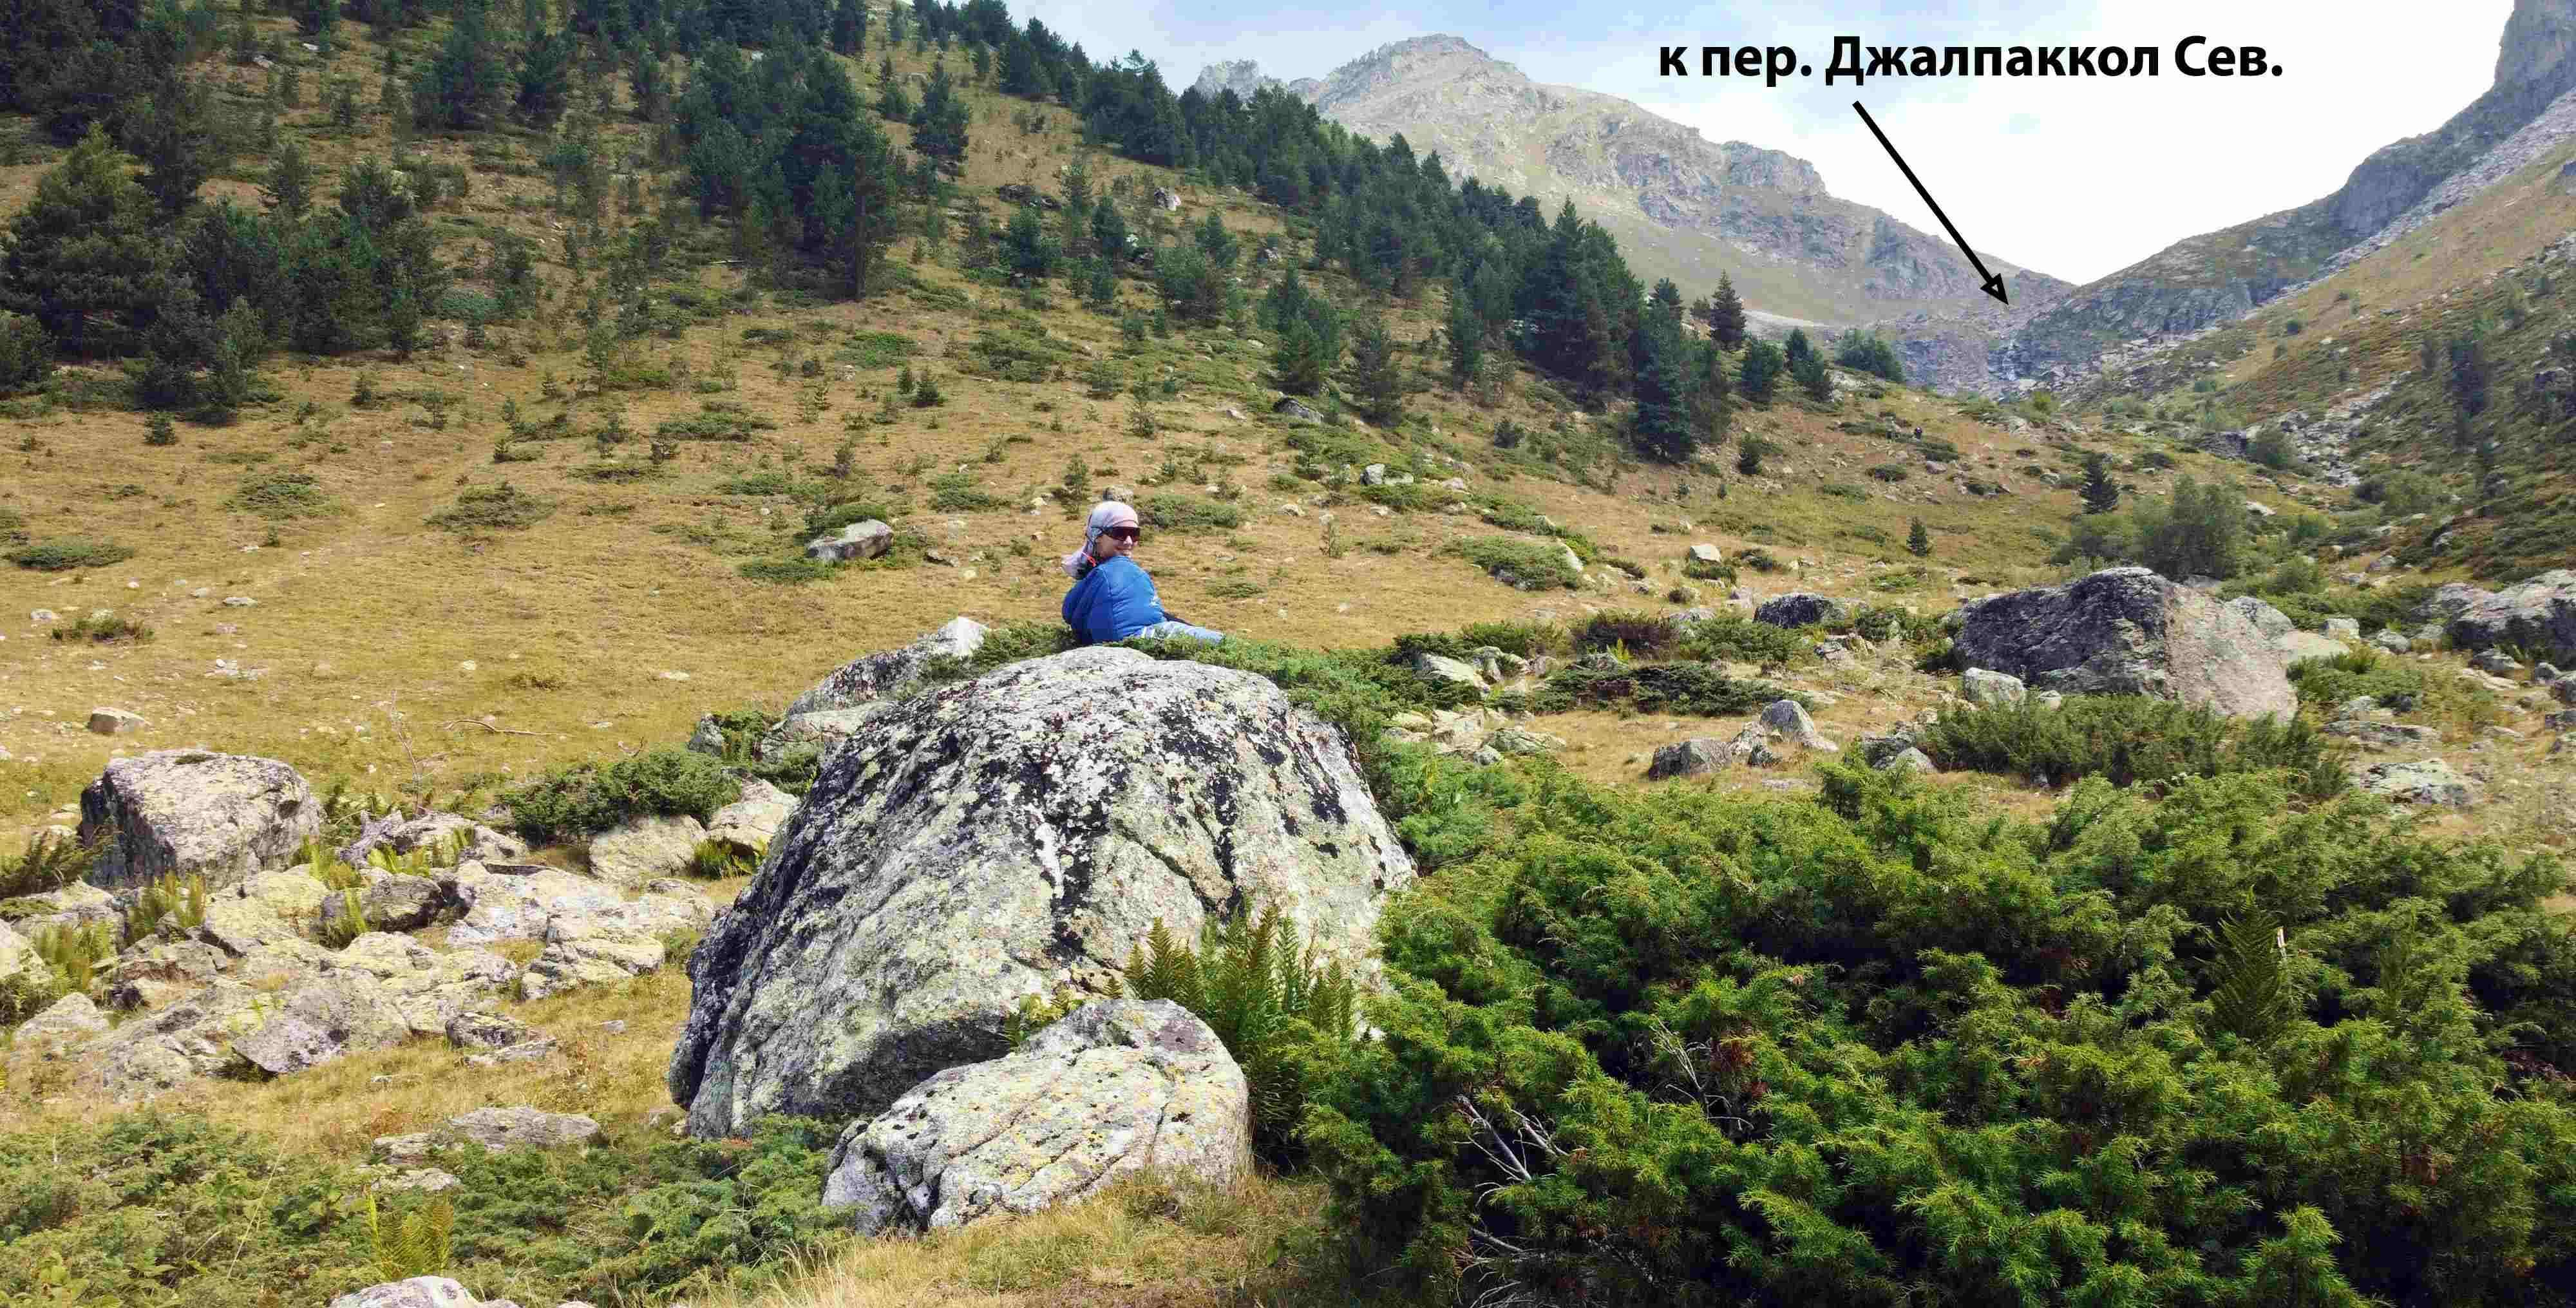
\includegraphics[width=0.7\linewidth]{../pics/DJI_0830}
	\caption{На фотопривале}
	\label{fig:DJI_0830}
\end{figure}

Далее следовали по хорошо набитой и промаркированной тропе по ущелью Кичкинекола Джалпаккольского. При подъёме на ту ступень долины, которая окачивается бараньими лбами и водопадами, обходили их слева пхд (рис. \ref{fig:DJI_0835}).


\begin{figure}[h!]
	\centering
	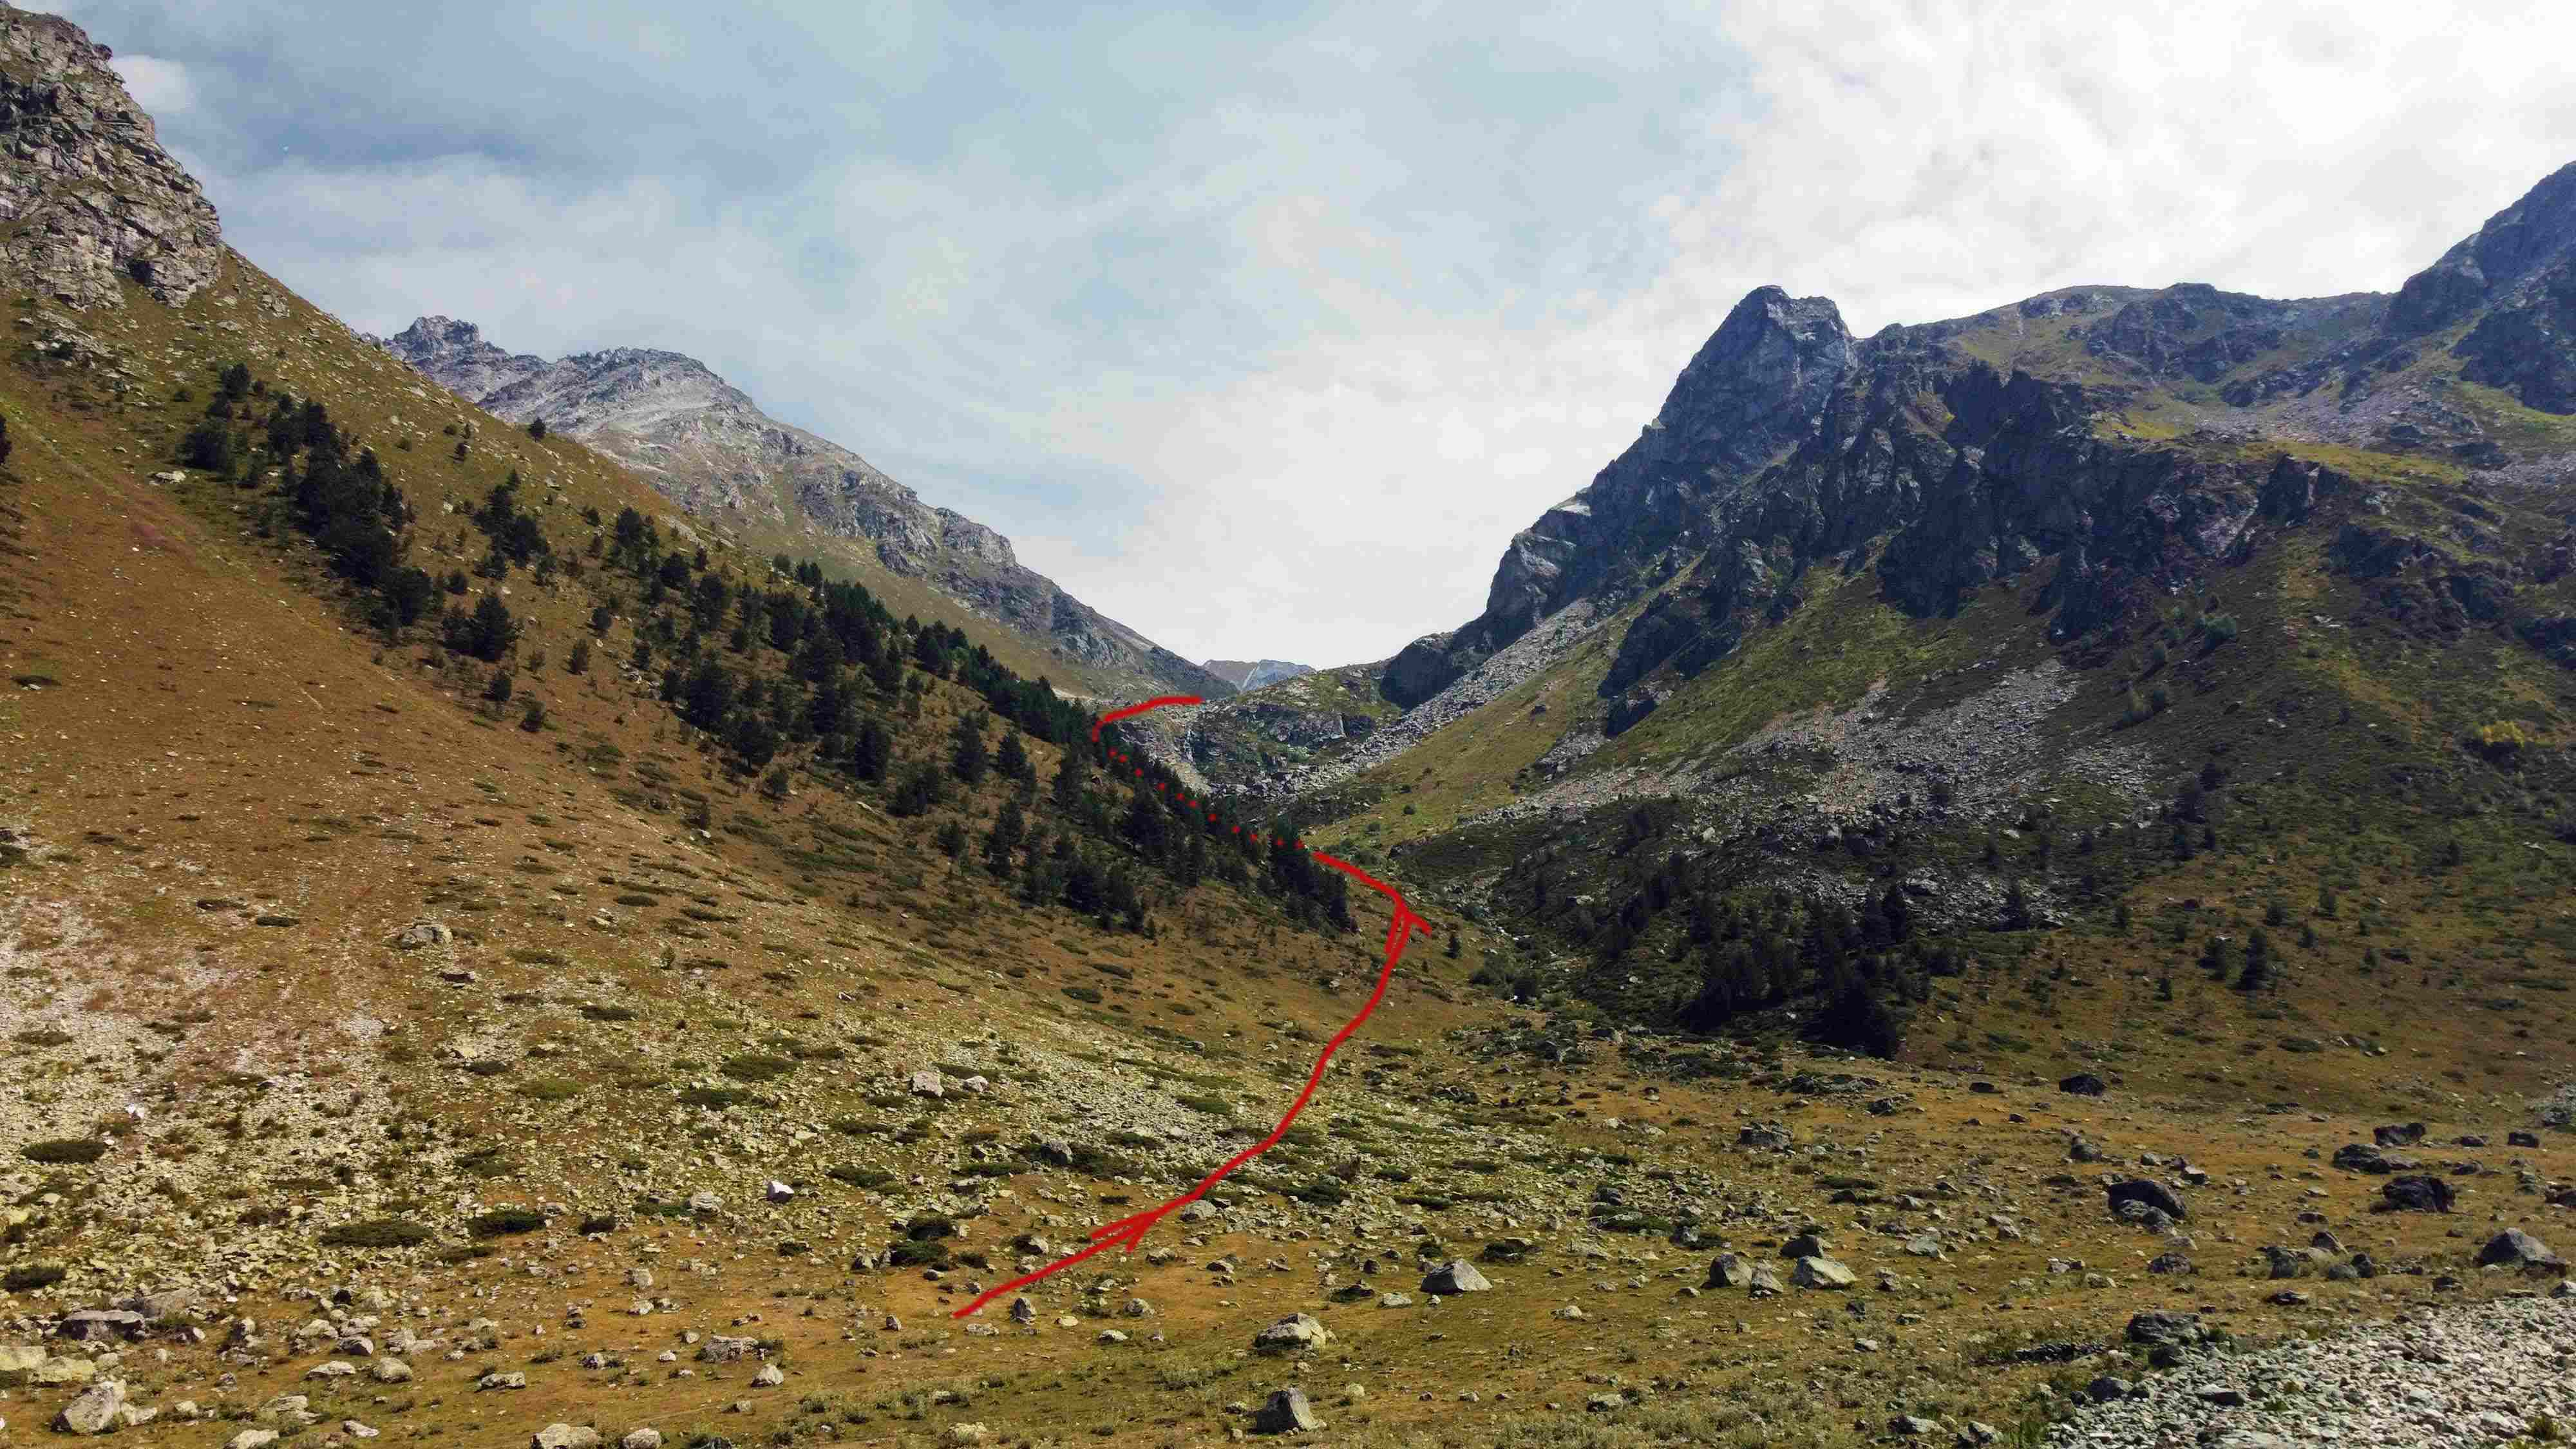
\includegraphics[width=0.7\linewidth]{../pics/DJI_0835}
	\caption{Маршрут подъёма в д.р. Кичкинекол Джалпаккольский из д.р. Джалпаккол}
	\label{fig:DJI_0835}
\end{figure}

За водопадами на древней морене нас обогнала группа коммерческих туристов. Инструктор группы удивился тому, что мы в рамках похода 1 к.с. идём перевал Джалпаккол Северный. 

Упомянутая древняя морена представляет из себя курумник с валунами впечатляющих размеров. Тропа, которой шли коммерческие туристы, и по которой шли затем мы, обходит его слева пхд, продолжая тем самым траекторию обхода бараньих лбов. С правой от курумника стороны тоже читается тропа, но вариант обхода слева выглядит более популярным. \alert{(Должна быть фотография: я специально просила Машу её сделать)}

Обойдя курумник, в 15:45 устроили обед на оборудованной стоянке (N~43.288482\degree,\\E~42.081736\degree). Дальнейший путь частично скрыт за моренным валом --- виден только крутой подъём на следующую ступень где-то в километре впереди, поэтому уверенности, что имеет смысл пытаться подойти к этой ступени, нет. Однако по итогам разведки, которую организовали во время обеда, выяснилось, что участок пути от ближайшего моренного вала до подножия ступени хороший: плоский, без паразитных сбросов, и представляет из себя разлив ручья, стекающего с пятиозёрья Куршо. Соответственно, было принято решение подойти к началу подъёма на ступень вплотную. Долину тем временем начало затягивать тучами, поэтому мы поторопились закончить с обедом и выдвинуться к окоончательному месту ночёвки (N~43.285565\degree, E~42.091178\degree, рис. \ref{fig:DSC_0018}), куда дошли в 18:30. Глубокой ночью (примерно с 01:00 по 03:00) разразилась сильная гроза с частыми молниями и сильным ливнем.

\begin{figure}[h!]
	\centering
	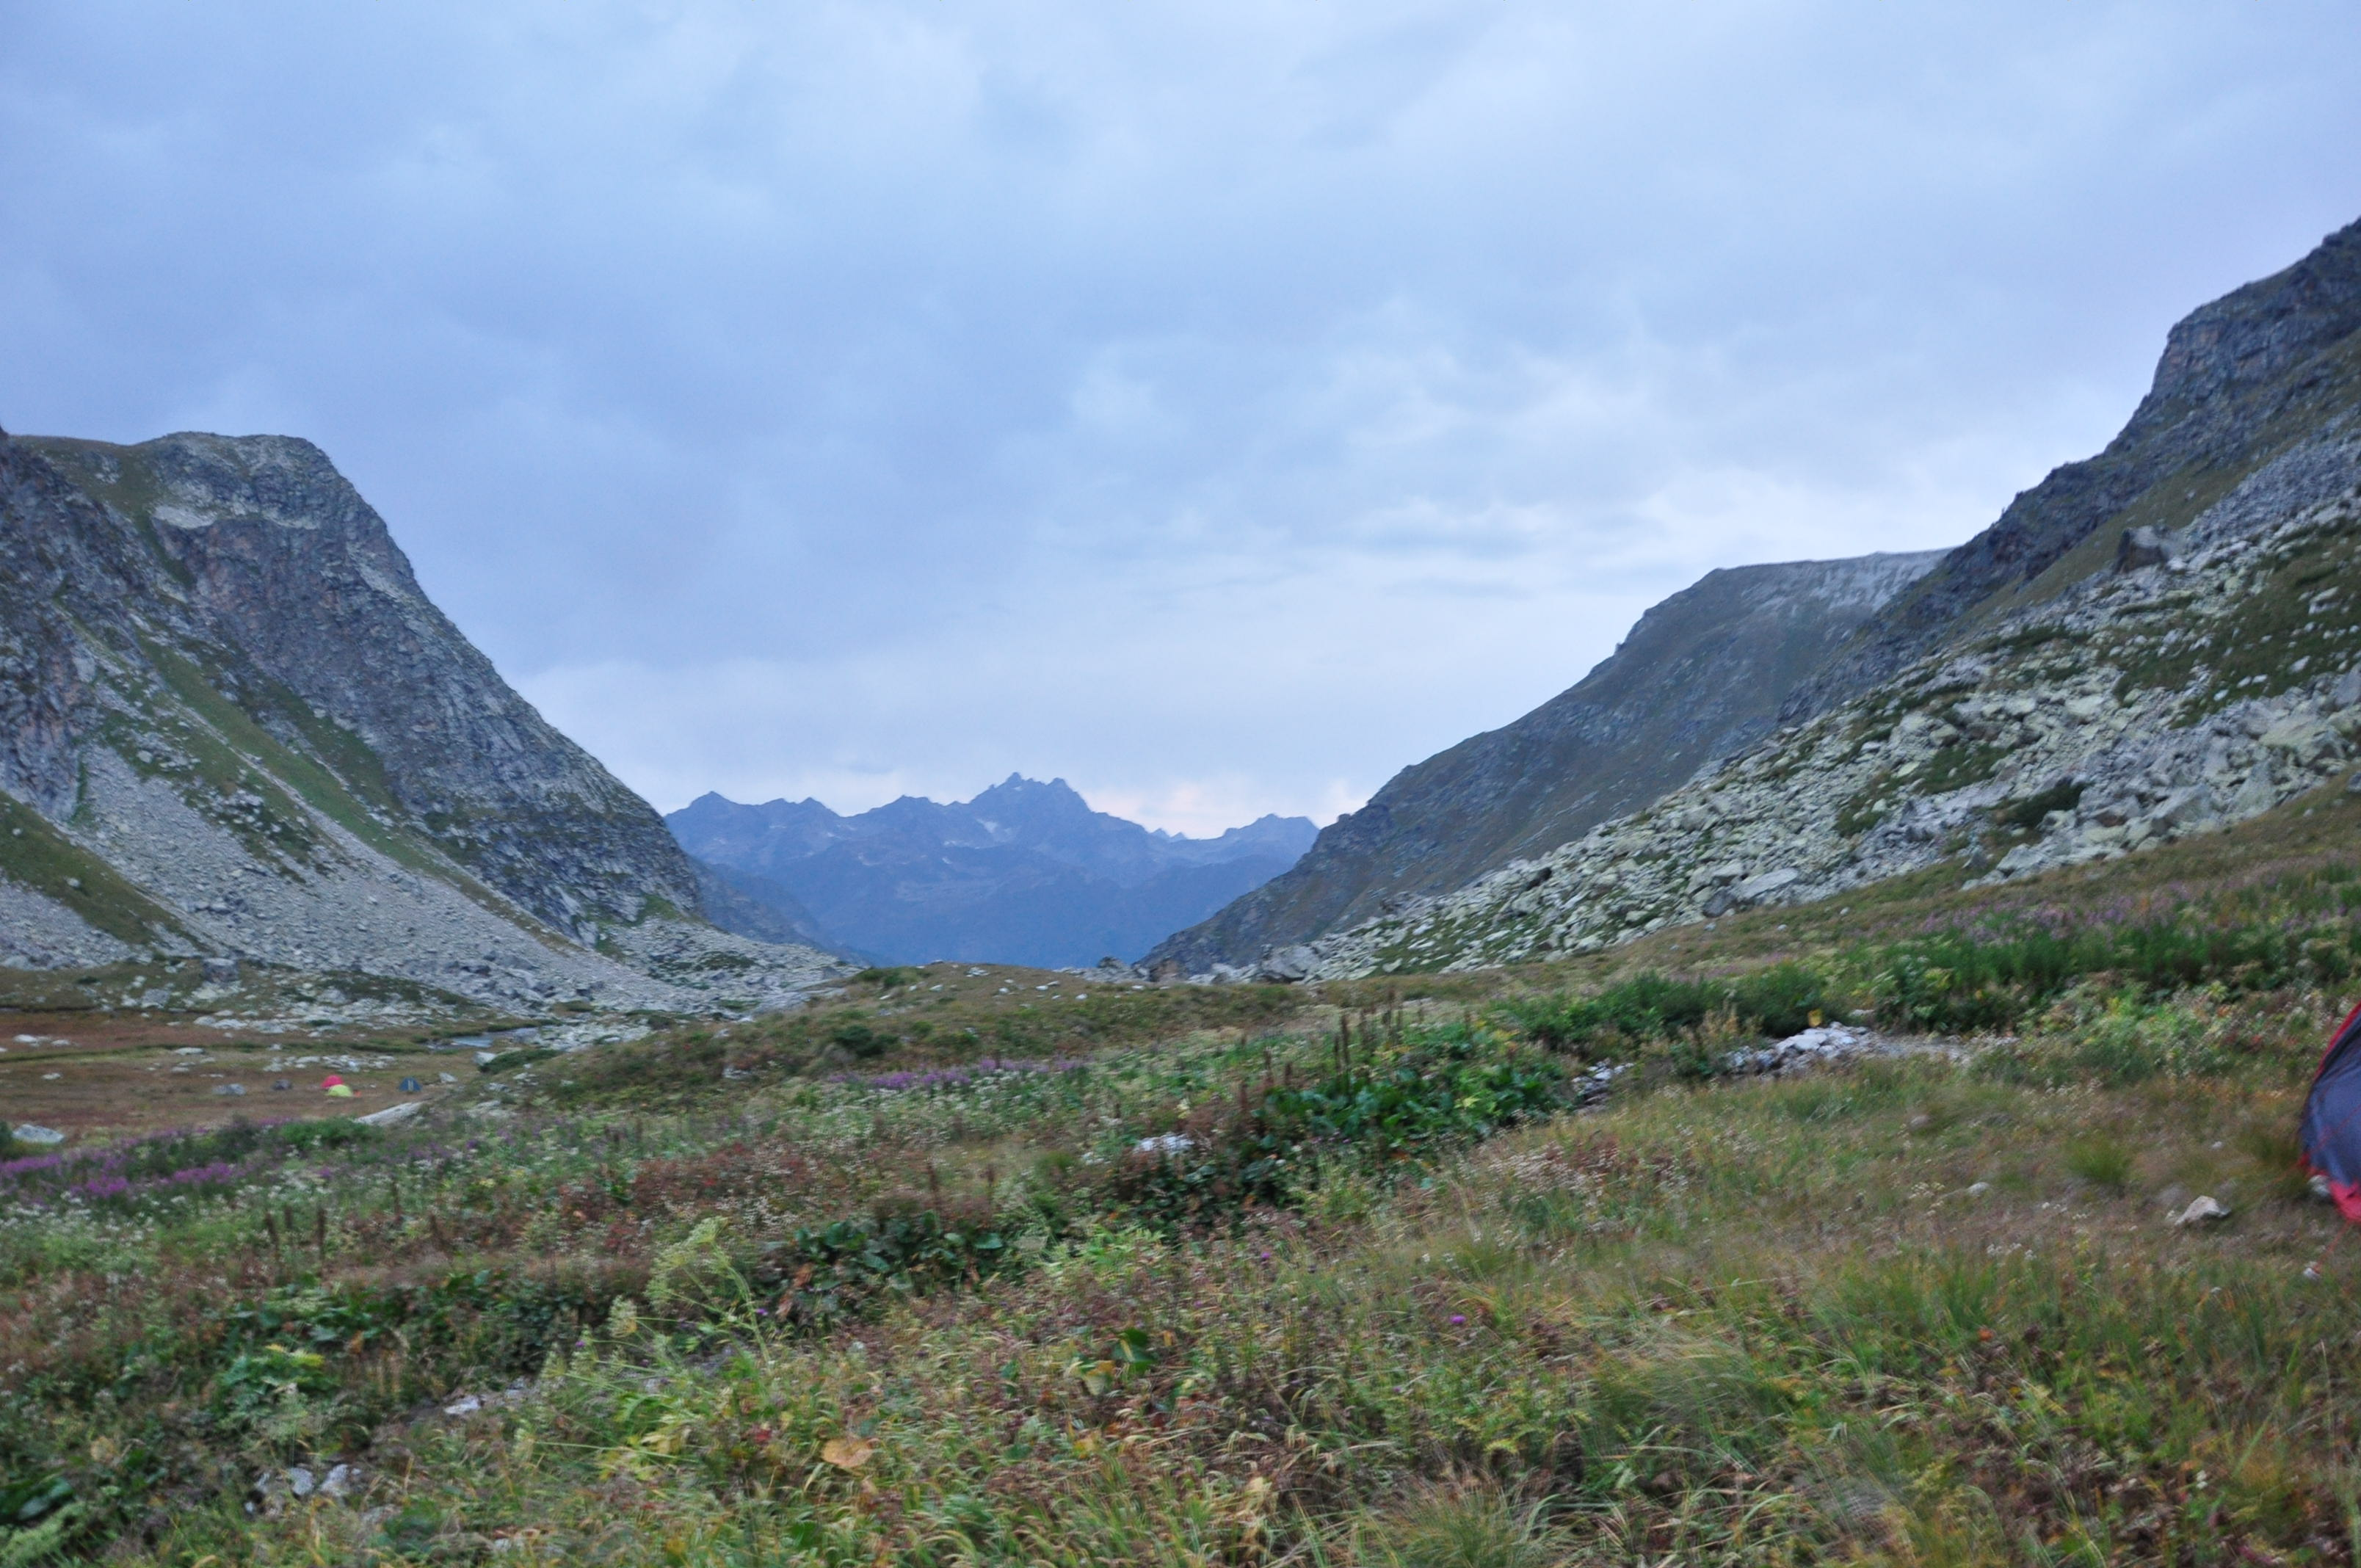
\includegraphics[width=0.7\linewidth]{../pics/DSC_0018}
	\caption{Место ночёвки 22-23.08}
	\label{fig:DSC_0018}
\end{figure}

\clearpage